\chapter{Challenges}
% Some challendges of showing/controlling clustered PROV
% Automatic clustering. 
% Naming. 
% False connections.

This clustering seems promising to reduce the size, and so, the complexity, of the visible provenance graph 
%% I altered this as it sounds passive but if the user actually did the action, that is very active
in an interface.
Many challenges remain about the ways to make the clustering interface work well for users, 
so they can do clustering, and then to explore the graph. This section discusses challenges we have encountered.

\section{Specification of user-defined clusters}
\label{sub:introduction_to_clustering}

A clustering action takes a set of nodes and combines them. 
Our interface follows the established interface method to select multiple items,
hold down \textit{ctrl} then click each node, once multiple nodes are selected a contextual link will appear in the details panel (like the blue links in Fig.~\ref{fig:fitness-grouped}) allowing the user to group them. 
This works well for combining a small number of nodes. 
When the user wants to combine a larger number of nodes, 
it would be useful to add a regular language, 
so the user can define a property for all the nodes to be clustered.
For example, suppose each day's Fitbit data was a separate node.
The user may want to cluster them to a single node,
with an expression such as ``cluster all the nodes where the name is `Fitbit-*-*-Jan-2016'.'' 
The language should be able to refer to a variety of node attributes, such as Date, Source, Type, etc.

This may go beyond just features of the node, to include the relationship between this node and others: 
for example, ``cluster all Fitbit nodes that are not used in a particular report.'' 
It may be useful to support parameterised clustering, 
where one command creates multiple clusters 
(for example, ``cluster all the Fitbit nodes from each month, separately, into a month-granularity cluster'). 
It will be challenging to design such a language, so that it is both powerful and easy to learn and use.
%
Some automation may help, with where the platform suggesting clusterings, based on workloads of provenance queries recorded (for example, one might cluster nodes which are frequently accessed together).

\section{Useful naming}

Once nodes have been clustered, it is difficult to automatically generate a name 
that the user will find meaningful for the new cluster~\cite{Schaffer1996, Abello2006}. 
Automating this process requires domain knowledge and it may also need deep models of the user and their needs.
This would be a substantial undertaking. 
For example, it may demand recognition that \textit{vim}, \textit{emacs} and \textit{nano} are all text editors? 
In an early version of our prototype, a new cluster-node was given a short random alpha-numeric name. 
However, this made the graph incomprehensible, with users needing to manually update the name immediately
so that they could understand the graph. 
Our current, still simple approach uses the name of the node in the cluster with the shortest distance from the root with the text ``group'' appended to the end. 
So, for example, in the transition from Figure~\ref{fig:fitness-ungrouped} to Figure~\ref{fig:fitness-grouped}, the node created would be named \textit{Fitness-Summary group}.


\section{Avoiding false dependencies}

Clustering is a simple type of graph rewriting, which creates an abstraction of the graph and in turn simplifies details of the original graph. This can produce false dependencies: these are newly implied lines of lineage, created by the clustering, and they falsely suggest that one entity had influence upon another. 
Worse yet, circular dependencies may occur, along with other violations of the constraints defined in the PROV-CONSTRAINT W3C document~\cite{w3c-prov-constraints}. For example, if the clustering set in the example of Fig.~\ref{fig:fitness-ungrouped} only included nodes \{\texttt{fitness-summary}, \texttt{CalorieIntakeFeed}\},  then a simple replacement of these nodes with a node $x$ would result in a circular dependency, namely $\langle x \; \mathtt{wasGeneratedBy} \; \mathtt{summarize}\rangle$ and $\langle \texttt{summarize} \; \texttt{used} \; x \rangle$, you can see this in Fig.~\ref{fig:loop}.
A theoretical formulation of provenance abstraction by \textit{grouping} (clustering) has been proposed in~\cite{Missier2014} to describe this and other problems that occur with clustering, along with simple algorithms for grouping arbitrary sets of nodes. 
Essentially, that work showed that to avoid false dependencies, as well as circular data dependencies, one must first compute a \textit{closure} operation that extends the user-selected nodes with all other nodes that sit on any path amongst these initial clustering nodes.
Combining this prior work with our user-oriented provenance navigation model can lead to a provably correct clustering mechanism. 
%A check could be made comparing suggested lineage of nodes around a cluster selecteion before and after a clustered node is created to see if any false connections exits. In some cases false connections may be desireable to obviscate sensitive information.

\begin{figure}[h]
	\centering
	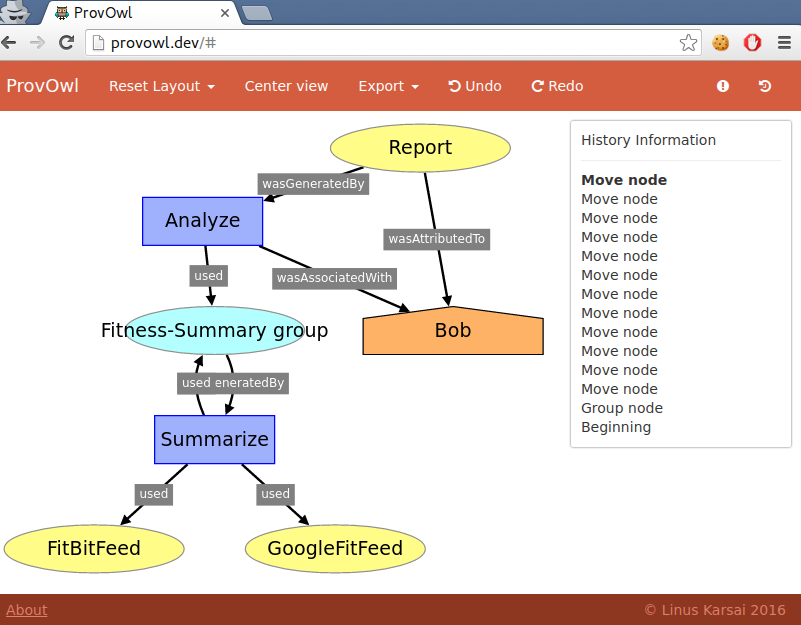
\includegraphics[width=\linewidth]{loop}
	\caption{When grouping on \{\texttt{fitness-summary}, \texttt{CalorieIntakeFeed}\} a circular dependency is caused between \texttt{Fitness-Summary group} and \texttt{Summarize}. The panel on the right can be toggled by the history button above and shows a list of user actions with the current state indicated in bold. Users can use the \textit{Undo} and \textit{Redo} buttons to move between actions.}
	\label{fig:loop}
\end{figure}


